\chapter{Introduction}
\label{sec:intro}
In the current years the amount of embedded devices has drastically increased. This is mostly due to the emergence of the Internet of Things (IoT), as well as the existence of several user friendly kits, like the RaspberryPi or the Arduino. However it is quiet complex to monitor and debug such devices, once they deployed. Even more difficult is it to monitor a whole WSN. In order to address this problem, three are different possiblities, e.g. the use of WSN testbed, which are attached to the sensor node and thus allow the node to be monitored.

Another problem of WSN, is the reconfiguration of the nodes once they are deployed, e.g. if the task the nodes fulfills changes. Most of the times, the nodes need to be collected and programmed one by one.

In order to address both those problem SHAMPU was developed. SHAMPU is a WSN testbed framework, which is attached to an exisiting node and is thus capable to not only monitoring the mote, but also to reprogram it. All SHAMPU devices are part of their own network and conenected to a base station, which acts as a master and controls all the SHAMPU nodes. The communication between the SHAMPU nodes is handle by and ANT chip.

In this thesis we evaluate that part of the SHAMPU framework and determine the capabilities and limitations of the ANT chip. Especially important are the amount of data which can be transfered inside the ANT network and the communication range of the network itself. To accuralty assess the ANT network, we design and run several experiments, which cover a wide range of use-cases.


\section{Related work}
\label{sec:related_work}

There are already several different WSN testbeds available. Each of these testbeds were designed to fulfill a different role. 

Some testbeds like FlockLab \cite{Lim2013} provide a wide array of  or Minerva \cite{Sommer} ....  However these testbeds rely on a fixed infrastructure, the node to be tested has to be directly connected to the testbed. This makes it difficult to test and debug already deployed WSN, since it might not be possible to attach the testbed to the nodes.

Other solutions use a WSN for the testbed itself. For examples Sensei-UU \cite{Rensfelt2009} use testbeds which are directly attached to the tested node and communicate the debugging info via wirless 802.11 networks. This allows the WSN to be tested and debugged while it is deployed. The powerdraw of 802.11 networks, compared to other technologies, like Bluetooth is huge. This makes it hard to run the nodes of a battery and without an external power source.



BTNodes \cite{Moser} or Smart-Its \cite{Kasten2000} use Bluetooth to address the power issue. But Bluetooth introduces different problems, such as size limitations for the network and a difficult set-up and use of more complex network topologies. The newest version of Bluetooth tries to address this with the introduction of ScatterNets, but the setup and maintenance of the network still remains challenging.


\chapter{Technical Background}
\section{SHAMPU}
SHAMPU (Single chip Host for Autonomous Mote Programming over USB) \cite{Smeets:2014:DAL:2602339.2602401} is a WSN testbed, which allows the remote debugging and reprogramming of sensor nodes. The main advantages over other testbeds (see section~\ref{sec:related_work}) are the portability, low cost, small size and low energy consumption. SHAMPU is and attachedment, which is used as an extension to an already existing sensor node. The node only needs to provide an USB-Interface, SHAMPU itself is completely OS independent.
\begin{figure}[h]
\centering
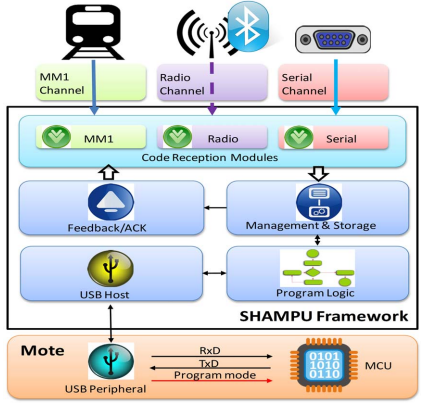
\includegraphics[scale=.5]{./pics/SHAMPUframework.png}
\caption{Overview of the SHAMPU Framework}\label{fig:shampuframework}
\end{figure}
The SHAMPU framework (see Figure \ref{fig:shampuframework}) itself is split into multiple modules. The Code Reception Module allows the use of different protocols to connect to and communicate with the SHAMPU device. For wireless communication SHAMPU uses an ANTAP1MxIB RF Transceiver Module, which supports the ANT protocol. The USB Host module is used to connect to the sensor node, which SHAMPU is attached to.

\section{ANT}
ANT \cite{DynastreamInnovationsInc.2013} is a wireless protocol which operates in the 2.4 GHz ISM Band. Originally developed in 2003 by Dynastream Innovations Inc. for the use wireless sensors. The ANT protocol is designed for the use in low power WSNs and puts a focus on scalability and ease of use.
\begin{figure}[h]
\centering
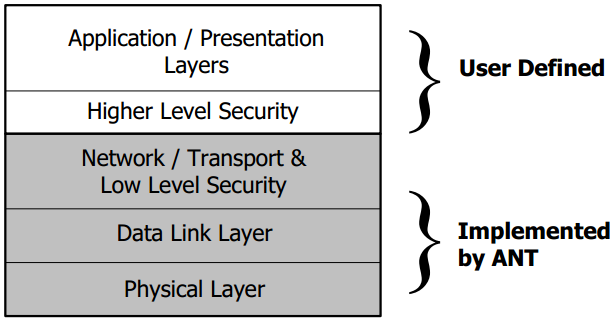
\includegraphics[scale=.5]{./pics/ANTstack.png}
\caption{OSI-Layer vs. ANT Protocol}\label{fig:osilayer}
\end{figure}
One of the advantages ANT has over other protocols, like Bluetooth or ZigBee is the high level of abstraction the ANT Protocol provides. This is achieved by the incorporation the first 4 OSI-layer (see Figure \ref{fig:osilayer}) into the ANT protocol and thus allowing even low-cost MCU to setup and maintain complex wireless networks.

\subsection{ANT Topology}
In order for the ANT protocol to work each mote needs to be part of a network. As shown in figure \ref{fig:anttopo} the ANT protocol can be used to create simple or more complex networks. Each mote inside a network is called an ANT node and in order for two nodes to communicate with each other they need to be connected via a channel.

\begin{figure}[h]
	\centering
	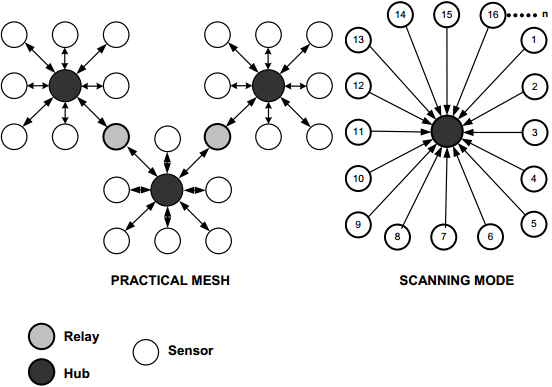
\includegraphics[scale=0.7]{./pics/ANTtopo.png}
	\caption{Example ANT Topologies}\label{fig:anttopo}
\end{figure}


\subsection{ANT Channels}
Most of the available channel types are bidirectional, but the ANT protocol still differentiates between master and slaves nodes. While a master nodes mostly sends data and a slave nodes mostly receives data, the slave still has the ability to response to the incoming data.

The ANT protocol knows 125 different channels, each 1 MHz wide. Each Channel supports a data rate of 1 Mbps and up to 65533 nodes. To avoid interference between the channels isochronous self adjusting TDMA technology is used, this allows the ANT nodes to change the transmit timings and even the frequency that is being used for the current channel.

\textit{Picture Process to establish a channel between master and slave nodes.}

The ANT protocol distinguishes between 2 different Channel types:
\begin{description}
\item{\textbf{Independent Channels}} \hfill \\ Independent Channels are used if there is only one node, which is transmitting data. There is no limit of the amount of slave devices, which receive the messages being send out. Furthermore the message being send out is broadcast to all nodes, it is not possible to only address a specific node.
\item{\textbf{Shared Channels}} \hfill \\ Shared Channels are used if a single ANT node needs to receive data from many nodes. This type of channel is made possible by the use of Shared Channel Address, however this reduces the amount of data that can be transmitted at a time. The Channel master can decided to either use one or two bytes as the address, which allows for either 255 or 65535 slave devices in the same channel.
\end{description}

\subsection{ANT Communication}

The ANT protocol supports 3 different data types: broadcast, acknowledge and burst. The data type is not part of the channel configuration and thus channels are able to use any combination of data types. The only exceptions are unidirectional channels, which can only ever send broadcast data. The different types of data types differ in how the data is handled and transmitted.

\begin{itemize}
	\item{Broadcast data} \hfill \\ Broadcast data is the most basic datatype and the default. To start a broadcast transmission, the command needs to be issued only once, since the last send packet is periodically resend as a broadcast. Even if the last packet was part of a burst or acknowledge transmission. Figure (xyxcy) shows, how each broadcast transmission is aligned to the channel message period.	Since there is no answer from the receiving node, it is not possible to determine if the packet was transmitted correctly or not.

	\item{Acknowledge data} \hfill \\ Acknowledge data can be used to make sure a node received a transmitted packet. After the reception of a acknowledge packet, the node will send a message back to the sender. Acknowledge data can only be used with bidirectional channels, however both the master and the slave can use it. Figure (Xyxy) shows that, just like broadcast acknowledge data is always aligned to a time slot, but the answer from the receiver is send immediately back to the sender.
	
	\item{Burst data} \hfill \\ Burst data provides a method to quickly transmit large amounts of data. This is achieved by ignoring the normal channel time slots and sending the packets right after each other. This allows for a transmission rate of up to 20 kbps, much higher than other data transmissions types. Similar to ackownledge data at the end of the transmission the sender is informed if the transfer failed or succeeded. The drawback of the methods is, that burst data is prioritized over all other transmissions and can interrupted other transmissions over the same channel.
\end{itemize}

\subsection{ANT messages}
In the ANT protocol each message has the in Figure \ref{fig:antmsg} specified basic format.
\begin{figure}[h]
	\centering
	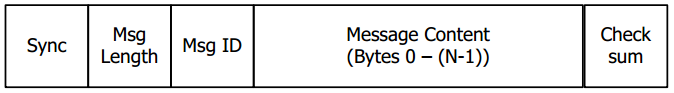
\includegraphics[scale=.75]{./pics/ANTmsg.png}
	\caption{Ant message structure}\label{fig:antmsg}
\end{figure}
Each message starts with a special Sync-Byte and end with a checksum, which is calculated by xoring all previous bytes. The Msg Length byte is the number ob Message Content bytes. The Msg ID byte specifies which kind of data is contained in the message. The ANT protocol also provides an extended message format, which allows to attached further information to each message.


\section{ANTAP1MxIB RF}
In order to use the ANT protocol each SHAMPU-mote is equipped with an ANTAP1MxIB RF Transceiver Module. The module was chosen because of it's small form factor (20mm x 20mm) and very low power draw. The ANTAP1M can handle up to 4 ANT channels with combined message rate between 0.5Hz and 200 Hz. and a 1Mbps RF data rate, which is enough to setup and use the desired network topology.

To more easily test the chip, we used a base-station for all the experiments. This basestation (see Figure XYXY) contains the ANTAP1MxIB and some other hardware, which allows the ANT to asynchronously communicate over RS-232 with a PC. 

\chapter{Evaluation of SHAMPU}
In order to assess the capabilities of SHAMPU we plan and run experiments designed to evaluate the SHAMPU framework according to the following use-cases:
\begin{itemize}
	\item{\textbf{Scheduled Data-transmission}} \hfill \\ In order for SHAMPU to work as a debugging and logging platform, the base-station needs to periodically receive data from all the nodes in the network. ANT provides two different data types which can be used to transport data in this case: Broadcast data and Acknowledge data. The Experiments designed for this use case try to determine the maximum throughput for each of the two transfer modes.
	\item{\textbf{Unscheduled Data-transmission}} \hfill \\ There are several possible cases, where its not feasible to use a scheduled data-transmission. Instead we use the burst mode, which allows to transmit data at a much higher rate. This use-case covers several different scenarios, e.g.:
	\begin{itemize}
		\item{}Reprogramming of a node: SHAMPU is able to reprogram the attached node. For this, it needs to receive a new firmware, which can be a couple MB big.
		\item{}SHAMPU RAM-Dumps: SHAMPU has 128kB of RAM, which can be used to collect data during an experiment. At the end the complete memory needs to be transmitted to the base-station.
	\end{itemize}
	\item{\textbf{Communication Range}} \hfill \\ Since SHAMPU is architecture independent it can be used in different situations. Thus it is important to know, how far away the nodes can be placed. In addition, since SHAMPU tries to be energy efficient, it might be viable to reduce the range for smaller setup to save even more energy.
\end{itemize}

For this we designed different experiments, which test one or more of the described categories. The following section describes the experiments according to the following template:

\begin{description}
\item{\textbf{Description}} \hfill \\ A description of the experiment and the the category being evaluated.
\item{\textbf{Use-Case}} \hfill \\ The use-case the experiment tries to test.
\item{\textbf{Network Topology and Configuration}} \hfill \\ A diagram of the network topology in which the experiment is run and the configuration of the complete network. Default values are not listed.
\item{\textbf{Testing methodology}} \hfill \\ A description on how the experiment is performed.
\item{\textbf{Result}} \hfill \\ The results of the experiment and any additional collected data.
\end{description}

\newpage

\section{Common Experiment parameters}

If not otherwise noted in the experiment description each Experiment were run in the Mobility lab of the Networked embedded Systems group at the University Duisburg-Essen (SA 327) and run with the following settings:
\begin{center}
\begin{tabular}{|c|c|}
	\hline Device Number & 33 \\ 
	\hline Device Type & 1 \\ 
	\hline Transmission Type & 1 \\ 
	\hline ID\_CHAN1 & 0 \\ 
	\hline FREQ\_CHAN1 & 2466 Hz \\ 
	\hline ID\_CHAN2 & 1 \\ 
	\hline FREQ\_CHAN2 & 2477 Hz \\ 
	\hline Message Period & 8192 \\ 
	\hline min\_Channel\_Period & 0x00A4 \\ 
	\hline max\_Channel\_Period & 0xFFFF \\ 
	\hline 
\end{tabular} 		
\captionof{table}{ANT default configuration}
\end{center}

Also there is an important difference between the message period used in the pseudo code and the frequency used in the figures, which display the results. The period describes the size of the gap between two messages, then frequency describes how many messages are send in 1 second. The channel period $p$ can be used to calculate the frequency of the time slots $f_t = \frac{32678}{p}$.  

\newpage


\section{Experiment 1: Broadcast Data Transfer between two nodes}
\begin{description} 
	\item{\textbf{Description}} \hfill \\ Broadcasting is one way to periodically transmit data between 2 or more ANT nodes. Since all broadcast packets are synchronized to a fixed time-slot, the data throughput can be increased by decreasing the channel period. However if the channel period is too small, the packets might start overlapping each other and interfere with the transmission. This experiment tries to find the smallest period with no interference.
	\item{\textbf{Use-Case}} \hfill \\ Scheduled Data-transmission	
	\item{\textbf{Network Topology and Configuration}} \hfill \\ \textit{Diagram for the experiment:  2 nodes} \\
		\begin{code}[h]
			\begin{verbatim}
			channelPeriod = max_Channel_Period
			while (channelPeriod >= min_Channel_Period) {
			  ANT_SetChannelPeriod(ID_CHAN1, channelPeriod)
			  ANT_OpenChannel(ID_CHAN1, ANT_Bidirectional_Master)
			  ANT_SendBroadcastData(ID_CHAN1, [0x01, 0x02, 0x03, 0x04])
			  wait_for_user_input()
			  ANT_CloseChannel(ID_CHAN1)
			  channelPeriod = decreaseChannelPeriod()
			}
			\end{verbatim}
			\caption{Master - Broadcast data transfer (1a)}\label{lst:mExp1}
		\end{code}
		
		\begin{code}[h]
			\begin{verbatim}
			channelPeriod = max_Channel_Period
			while (channelPeriod >= min_Channel_Period) {
			  ANT_SetChannelPeriod(ID_CHAN1, channelPeriod)
			  ANT_OpenChannel(ID_CHAN1, ANT_Bidirectional_Slave)
			  count = 0
			  for (10 seconds) 
			    if (receivedPacket() == ANT_BROADCAST_DATA)
			      count++;			  
			  print (count * 8 / 10) + " Bytes per second"
			  wait_for_user_input()
			  ANT_CloseChannel(ID_CHAN1)
			  channelPeriod = decreaseChannelPeriod()
			}
			\end{verbatim}
			\caption{Slave - Broadcast data transfer (1a)}\label{lst:sExp1}
		\end{code}	
	\item{\textbf{Network Topology and Configuration}} \hfill \\ The 2 nodes are placed right next to each other.
	 \item{\textbf{Testing methodology}} \hfill \\Node A acts as the master and node B as the slave. For both nodes the channel period is set to the highest value and the channel is opened. Node B records how many bytes it received over a 10s interval. The measurement is repeated 10 times and the average value saved. Then the channel period is decreased and the process repeated.
	\item{\textbf{Result}} \hfill \\  
	\begin{figure}[h]
	\centering
	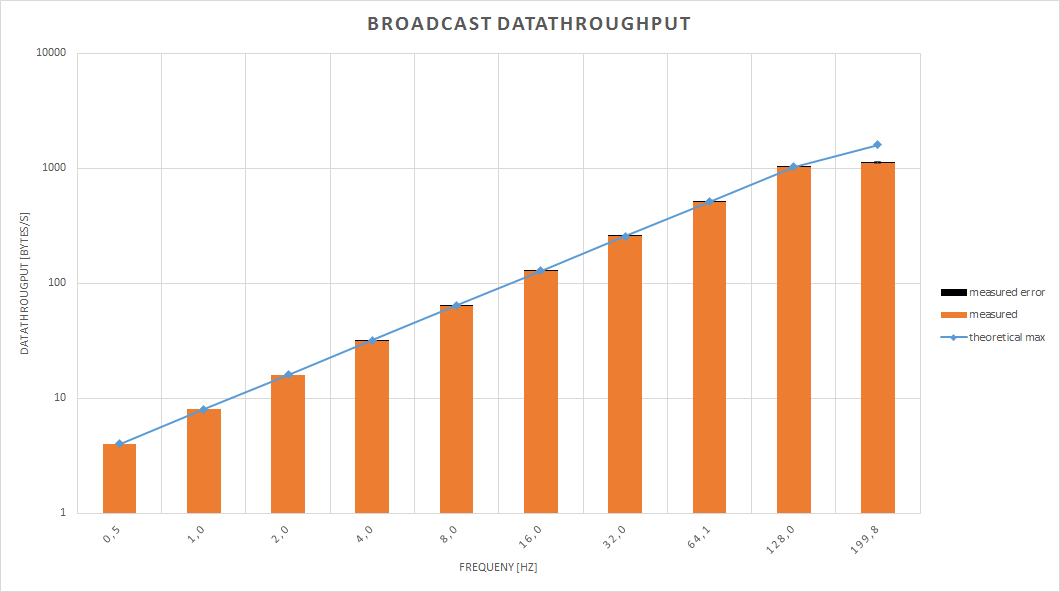
\includegraphics[scale=0.5]{./pics/exp1_norm.png}
	\caption{Broadcast datarate}\label{fig:exp1norm}
	\end{figure}
	
	Figure \ref{fig:exp1norm} shows the achieved transmission speeds for the different frequencies. Up a frequency of 128 Hz the measured data rate, matches the expected theoretical maximum rate. For the highest supported frequency (200 Hz), the measured data rate is much lower the the maximum rate. Even accounting for transmission errors the difference can't be fully explained. 
		\begin{figure}[h]
			\centering
			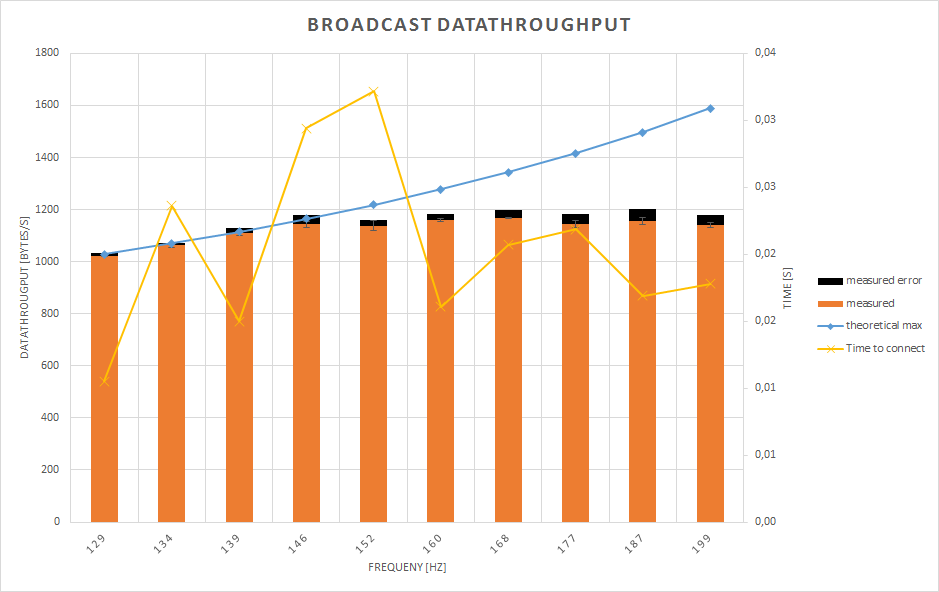
\includegraphics[scale=0.5]{./pics/exp1_detail.png}
			\caption{Broadcast datarate}\label{fig:exp1between}
		\end{figure}
	\newpage
	As seen in figure \ref{fig:exp1between} the measured data rates for frequencies above 140 Hz all fall short of the expected values. However the average of these frequencies is consistant at around 1100 Bps. The experiment was repeated multiple times, at different times and places and thus an environmental factor can be discarded. That means that the reason for the upper limit has to be with the hardware itself. See section \ref{sec:dataThrougput} for a discussion about possible reasons for this upper limit.				
\end{description}
\newpage

\section{Experiment 2: Broadcast Data Transfer between multiple nodes}
\begin{description} 
	\item{\textbf{Description}} \hfill \\ In Experiment 1 we determined the channel period, which allows for the maximum throughput. In this experiment we try to determine, how this value is affected by the amount of channels in the network. SHAMPU needs two channels, to work correctly: One channel, which sends data from the base station to the nodes in order to control them, and another channel with which the nodes can send information and debugging informations back.
	\item{\textbf{Use-Case}} \hfill \\ Scheduled Data-transmission	
	\item{\textbf{Network Topology and Configuration}} \hfill \\ \textit{Diagram for the experiment:  2 nodes} \\
		\begin{code}
			\begin{verbatim}
			channelPeriod = max_Channel_Period
			while (channelPeriod >= min_Channel_Period) {
		      ANT_SetChannelPeriod(ID_CHAN1, channelPeriod)
		      openChannel(ID_CHAN1, ANT_Bidirectional_Master)
		      ANT_SendBroadcastData(ID_CHAN1, [0x01, 0x02, 0x03, 0x04])
   		      ANT_SetChannelPeriod(ID_CHAN2, channelPeriod)
   		      openChannel(ID_CHAN2, ANT_Bidirectional_Slave)
			  count = 0
			  for (10 seconds) 
			    if (receivedPacket() == ANT_BROADCAST_DATA)
			      count++			
			  print (count * 8 / 10) + " Bytes per second"
			  wait_for_user_input()
			  ANT_CloseChannel(ID_CHAN1)
			  ANT_CloseChannel(ID_CHAN2)
			  channelPeriod = decreaseChannelPeriod()
			}
			\end{verbatim}
			\caption{Master - Broadcast data transfer with two channels }\label{lst:mExp2}
		\end{code}
		
		\begin{code}
			\begin{verbatim}
			channelPeriod = max_Channel_Period
			while (channelPeriod >= min_Channel_Period) {
			  ANT_SetChannelPeriod(ID_CHAN1, channelPeriod)
			  openChannel(ID_CHAN1, ANT_Bidirectional_Slave)
			  ANT_SetChannelPeriod(ID_CHAN2, channelPeriod)
			  openChannel(ID_CHAN2, ANT_Bidirectional_Master)
			  ANT_SendBroadcastData(ID_CHAN2, [0x01, 0x02, 0x03, 0x04])
			  count = 0
			  for (10 seconds) 
			    if (receivedPacket() == ANT_BROADCAST_DATA)
			      count++			
 			  print (count * 8 / 10) + " Bytes per second"
			  wait_for_user_input()
			  ANT_CloseChannel(ID_CHAN1)
			  ANT_CloseChannel(ID_CHAN2)
			  channelPeriod = decreaseChannelPeriod()
			}
			\end{verbatim}
			\caption{Master - Broadcast data transfer with two channels }\label{lst:mExp2}
		\end{code}
 
	\item{\textbf{Network Topology and Configuration}} \hfill \\ The 2 nodes are placed right next to each other.
	\item{\textbf{Testing methodology}} \hfill \\ In this experiment each nodes acts as a master for a different channel. Node A is the master for Channel 0 and Node B is the master for Channel 1. The measurements itself are identically to experiment 1, except that the data is recorded on both Nodes. The channelPeriod is decreased until the data throughput drops, or the connection can no longer be established.
	\item{\textbf{Result}} \hfill \\  	
	\begin{figure}[h]
		\centering
		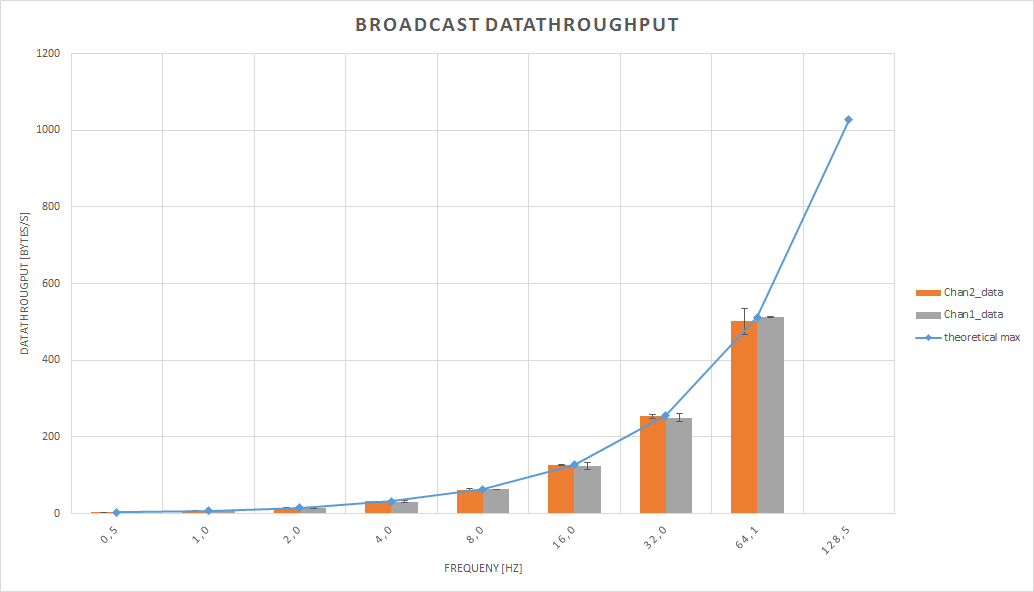
\includegraphics[scale=0.5]{./pics/exp2_norm.png}
		\caption{Broadcast data through - 2 channels}\label{fig:exp2low}
	\end{figure}
	\begin{figure}[h]
		\centering
		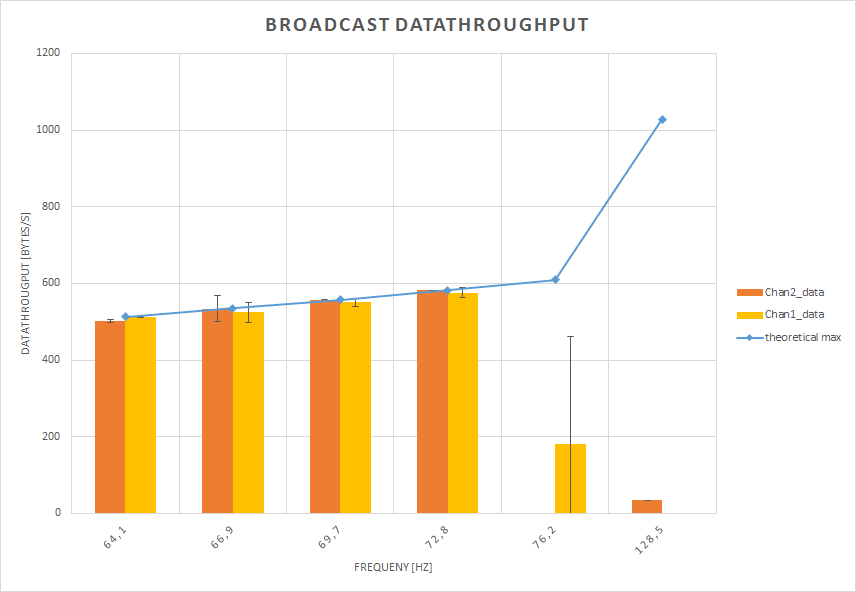
\includegraphics[scale=0.5]{./pics/exp2_detail.png}
		\caption{Broadcast data through - 2 channels}\label{fig:exp2high}
	\end{figure}
	Figures \ref{fig:exp2low} shows the results of the measurements, the left bar displays the throughput for channel 0, the right bar displays the throughput for channel 1. The blue line show the theoretical maximum of the data throughput, for the given frequency. Up to a frequency of 64 Hz the data throughput increases with the frequency for both channels. However there is a complete drop at 128 Hz. Figure \ref{fig:exp2high} shows that somewhere between 72 Hz and 76 Hz the data throughput begins to cut off. The combined data rate for two channels in thus around 1160 Bps, which is in line with the result from experiment 1. From this data we can assume, that the whole available datarate of 1160 Bps, is simply split among all existing channels.
\end{description}
\newpage
\newpage


\section{Experiment 3: Acknowledge Transfer delay}
\begin{description} 
	\item{\textbf{Description}} \hfill \\ In this experiment we try to determine the time it takes for a node to received and acknowledge a transmitted packet. This value is important for the control of the nodes in the network. ...
	\item{\textbf{Use-Case}} \hfill \\ Scheduled Data-transmission
	\item{\textbf{Network Topology and Configuration}} \hfill \\ \textit{Diagram for the experiment:  2 nodes} \\
	\begin{code}
		\begin{verbatim}
		channelPeriod = max_Channel_Period
		while (channelPeriod >= min_Channel_Period) {
		  ANT_SetChannelPeriod(ID_CHAN1, channelPeriod);
		  ANT_OpenChannel(ID_CHAN1, ANT_Bidirectional_Master);
		  duration = 0.0
		  for (i in 0..10) {
		    ANT_SendAcknowledgedData(ID_CHAN1, [0x01, 0x02, 0x03, 0x04])
		    start = getTime()	   
		    wait_for_ack()		
		    print (getTime() - start) + " s"	  
		  }
		  ANT_CloseChannel(ID_CHAN1)		
		  channelPeriod = decreaseChannelPeriod()
		} 
		\end{verbatim}
		\caption{Master - Acknowledge data delay}\label{lst:mExp3}
	\end{code}
	
	\begin{code}
		\begin{verbatim}
		channelPeriod = max_Channel_Period
		while (channelPeriod >= min_Channel_Period) {
		  ANT_SetChannelPeriod(ID_CHAN1, channelPeriod);
		  ANT_OpenChannel(ID_CHAN1, ANT_Bidirectional_Slave);				 
		  wait_for_user_input();
		  ANT_CloseChannel(ID_CHAN1);
		  channelPeriod = channelPeriod >> 1;
		}
		\end{verbatim}
		\caption{Slave - Acknowledge data delay}\label{lst:sExp3}
	\end{code}
	
	\item{\textbf{Testing methodology}} \hfill \\ Node A acts as the master and node B as the slave. For both nodes the channel period is set to the highest value and the channel is opened. Node A then sends a total of 10 acknowledge messages, and measured how long it takes until if receives the acknowledge signal. The channel period is then decreased and the experiment repeated.
	\item{\textbf{Result}} \hfill \\  
	\begin{figure}[h]
		\centering
		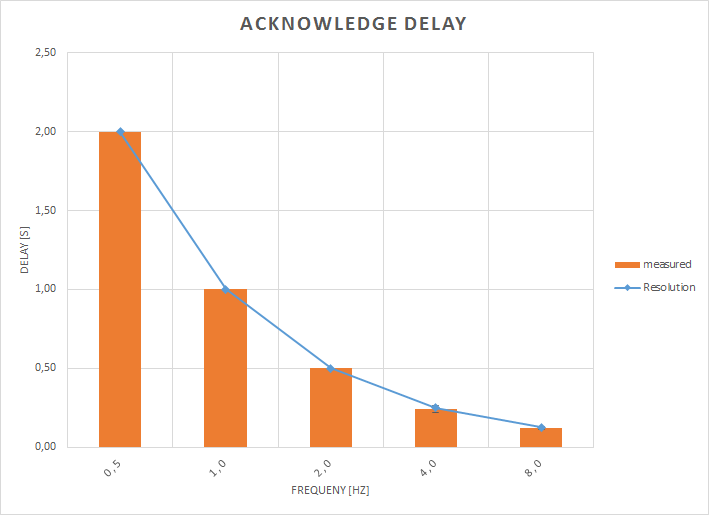
\includegraphics[scale=0.5]{./pics/exp3_norm.png}
		\caption{Burst delaye}\label{fig:exp3low}
	\end{figure}
		\begin{figure}[h]
			\centering
			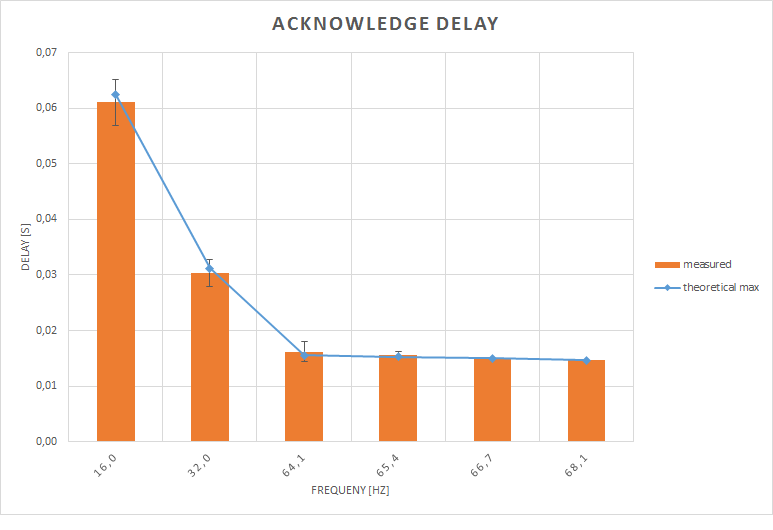
\includegraphics[scale=0.5]{./pics/exp3_detail.png}
			\caption{Burst delay}\label{fig:exp3high}
		\end{figure}
	Figure \ref{fig:exp3low} and Figure \ref{fig:exp3high} show the delays for the tested frequencies. The blue line shows the size between two timeslots, and can act as a resolution for each measurement. For the lower frequencies the results are skewed, since each acknowledge packet is aligned to a time-slot and thus the biggest part of the delay is waiting for the next time-slot. For frequencies greater than 64 Hz the data is much more useful, since the resolution is much lower than the measured values. The delay for those frequencies is around 18 ms, which no notable difference between 128 Hz and 200 Hz. 
\end{description}
\newpage


\section{Experiment 4: Acknowledge Data Transfer between two nodes}
\begin{description} 
	\item{\textbf{Description}} \hfill \\ This experiment is almost the same as experiment 1. The main difference is that we use acknowledge data instead of broadcast. It is also important to note that the master records how many successful packets are transmitted. The main goal of the experiment is, to see if the data throughput is decreased compared to broadcast data, especially for smaller channel periods.
	\item{\textbf{Use-Case}} \hfill \\ Scheduled Data-transmission
	\item{\textbf{Network Topology and Configuration}} \hfill \\ \textit{Diagram for the experiment:  2 nodes} \\
	\begin{code}
		\begin{verbatim}
		channelPeriod = max_Channel_Period
		while (channelPeriod >= min_Channel_Period) {
		  ANT_SetChannelPeriod(ID_CHAN1, channelPeriod)
		  ANT_OpenChannel(ID_CHAN1, ANT_Bidirectional_Master)
		  count = 0
		  for (10 seconds) {
		    ANT_SendAcknowledgedData(ID_CHAN1, [0x01, 0x02, 0x03, 0x04])	   
		    wait_for_ack()
		    count++
		  }
		  print (count * 8 / 10) + " Bytes per second"	  
		  ANT_CloseChannel(ID_CHAN1)
		  channelPeriod = decreaseChannelPeriod()
		} 
		\end{verbatim}
		\caption{Master - Acknowledge data transfer}\label{lst:mExp4}
	\end{code}
			
	\begin{code}
		\begin{verbatim}
		channelPeriod = max_Channel_Period
		while (channelPeriod >= min_Channel_Period) {
		  ANT_SetChannelPeriod(ID_CHAN1, channelPeriod)
		  ANT_OpenChannel(ID_CHAN1, ANT_Bidirectional_Slave)
		  wait_for_user_input()
		  ANT_CloseChannel(ID_CHAN1)
		  channelPeriod = channelPeriod >> 1
		}
		\end{verbatim}
		\caption{Slave - Acknowledge data transfer}\label{lst:sExp4}
	\end{code}
	\item{\textbf{Testing methodology}} \hfill \\ The testing methodology is the same as experiment 1a, except that the master sends acknowledge messages and waits for the slave to confirm the successful transmission before sending the next packet. 
	\item{\textbf{Result}} \hfill \\
	\begin{figure}[h]
		\centering
		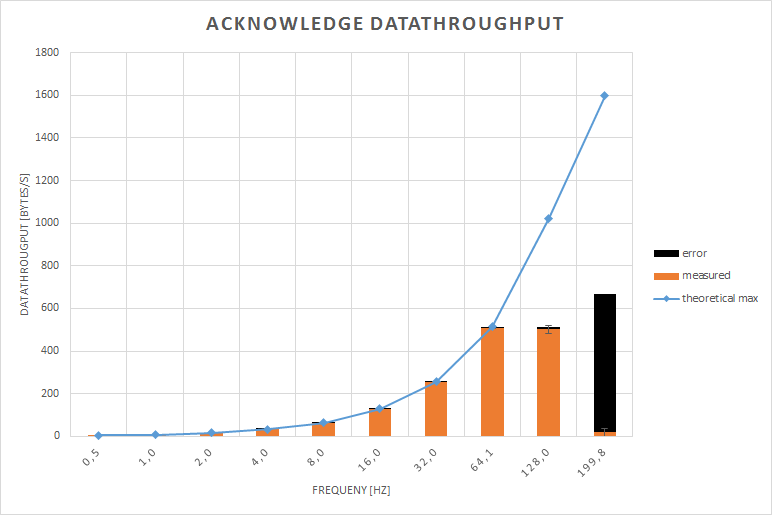
\includegraphics[scale=0.5]{./pics/exp4_norm.png}
		\caption{Burst datarate}\label{fig:exp4norm}
	\end{figure}
	Figure \ref{fig:exp4norm} shows the measured transmission speeds for the different tested frequencies. For the lower frequencies, the values align very well the with maximum data rate. Noteable however is the sharp dropoff at 128 Hz and the huge amount of incorrect transmission at 200 Hz. Figure \ref{fig:exp4between} show that every tested frequency between 128 and 200 Hz produces huge amount of transmission failures. Both observations can be explained with the results of experiment 3. The delay of an acknowledge message is roughly 18 ms. The problem is that ANT retransmits the last sent packet as a broadcast packet, if the frequency for this retransmission is too high it can interfere with the acknowledge message that the slave sends back to the master. For example at 200 Hz the message is broadcast every 5 ms resulting in too much data for the channel to handle. The transmission is thus interrupted. Since there is no increase of the data throughput between 64 Hz and 128 Hz, but a huge drop off at 133 Hz it can be assumed that some where around 128 Hz the channel is at the maximum data throughput of around 1100 Bps.
	\begin{figure}[h]
		\centering
		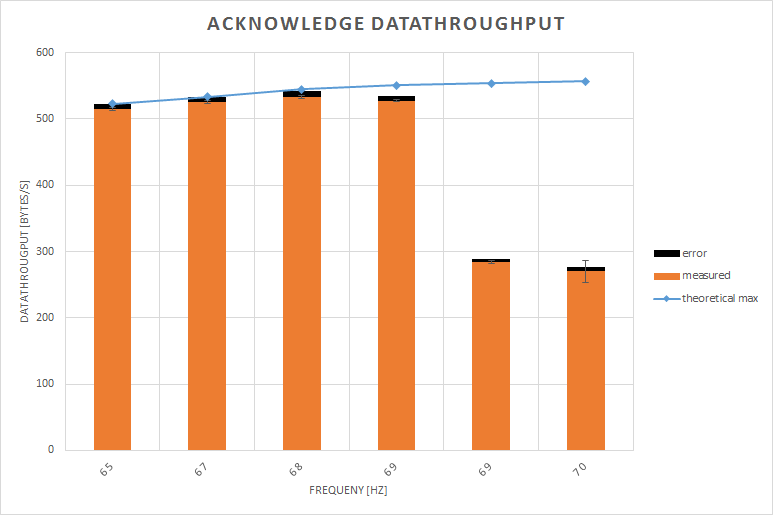
\includegraphics[scale=0.5]{./pics/exp4_detail.png}
		\caption{Burst datarate}\label{fig:exp4between}
	\end{figure}
\end{description}
\newpage


\section{Experiment 5: Burst Data Transfer between two nodes}
\begin{description} 
	\item{\textbf{Description}} \hfill \\ Burst data tranmissions make it possible to drastically increase the throughput rate. This allows a SHAMPU base station to quickly transmit a new firmware to a node or a node to dump its RAM back to the base-station.	According to the ANT specification promisses rates of up to 20 kbps can be achieved. To fully utilize this speed a baud rate of 50000 is needed. Since we are using 19200 baud we expect the maximum speed to be less than 20 kbps. We also try to determine, if the size of the burst transfer has an impact on the speed, since longer burst can disrupt communications on other channels.
	\item{\textbf{Use-Case}} \hfill \\ Unscheduled Data-transmission
	\item{\textbf{Network Topology and Configuration}} \hfill \\ \textit{Diagram for the experiment: PC with ANTUSB-m stick and 1 Node} \\

	\begin{code}
		\begin{verbatim}
		size = START_SIZE
		ANT_OpenChannel(ID_CHAN1, ANT_Bidirectional_Slave);		
		while (size >= END_SIZE) {
		  for (i in 0..10) {
		    wait_for_first_burst_packet()
		    start = getTime()
		    wait_for_last_burst_packet()
		    print (getTime() - start) / size " Bytes per second"
		  }
		  size = 2 * size
		}
		\end{verbatim}
		\caption{Slave - Burst data transfer}\label{lst:sExp5}
	\end{code}
	\item{\textbf{Testing methodology}} \hfill \\ Since the burst transmission mode, of our ANT-library is not working correctly (see section \ref{sec:future}) we use an ANTUSB-m Stick, which acts as a master. Node B is a normal base station and receives the burst transfers. Each different sized packet is send 10 times and the values recorded. The size is then doubled and the experiment repeated.
	\item{\textbf{Result}} \hfill \\ 
		\begin{figure}[h]
			\centering
			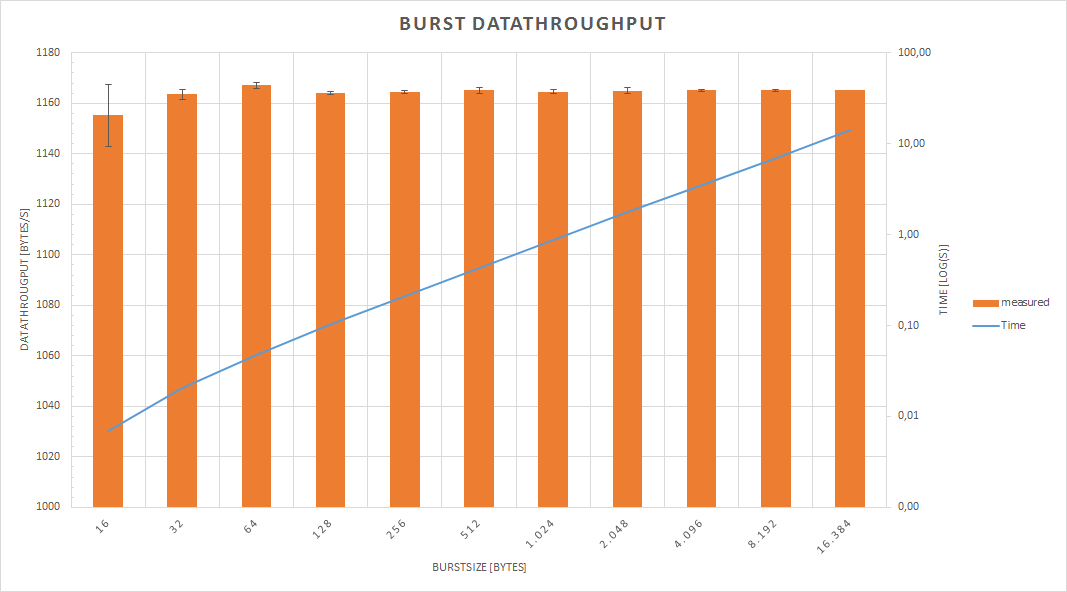
\includegraphics[scale=0.5]{./pics/exp5.png}
			\caption{Burst datarate}\label{fig:exp5}
		\end{figure}
	 Diagram (x) shows the transmission speeds for each of the different set ups.
\end{description}
\newpage

\section{Experiment 6: Maximal communication Range}
\begin{description} 
	\item{\textbf{Description}} \hfill \\  In this experiment we try to determine the correlation between the maximum range and the power setting of the ANT radio. One of SHAMPU's advantages is the low power consumption, so it might be possible to further reduce the power consumption by decreasing the power level of the ANT radio, especially in smaller environments where there is no need for such a long range.
	According to the datasheet the maximum range for communication is 30m, however the ANT documentation doesn't specify for which power setting this range can be achieved. 

	\item{\textbf{Use-Case}} \hfill \\ Communication Range		
	\item{\textbf{Network Topology and Configuration}} \hfill \\ \textit{Diagram for the experiment:  2 nodes   x meter apart.  with distances from 0.5 m to 30m  (floor in SM 3xx is 27m long)  A node is master, B node is slave. Node B is set up on a movable platform.}\\  

	\item{\textbf{Testing methodology}} \hfill \\ At the beginning of the experiment Node A and B are placed right next to each other. Node A acts as a master and keeps broadcasting the same message. Node B is the slave and tries to receive the broadcast message of Node A. After 20 broadcast messages are send, the transmission failures and successes are recorded and the distance between the two nodes is increased by 0.5 meters. This process is repeated until there are more failed than successful transmissions. At this point the distance is no longer increased, but decreased until there are more successful than failed transmissions. The whole experiment is then repeated for each available power setting.
	
	\begin{code}
		\begin{verbatim}
		for (pSetting in Available_PowerSettings) {
		  ANT_SetTransmitPower(pSetting)
		  openChannel(ID_CHAN1, ANT_Bidirectional_Master)
		  ANT_SendBroadcastData(ID_CHAN1, [0x01, 0x02, 0x03, 0x04])
		  wait_for_user_input();
		  closeChannel(ID_CHAN1);
		}
		\end{verbatim}
		\caption{Master - max communication range}\label{lst:mExp6}
	\end{code}
	
	\begin{code}
		\begin{verbatim}
		distance = 0, count = 0, fail = 0, success = 0
		stopInc = false
		openChannel(ID_CHAN1, ANT_Bidirectional_Slave)
		loop {
		  while (count < 20) {
		    receivePacket()
		    count++
		    if (transmission_Failed) fail++
		    else success++
		  }
		  if (stopInc) { 
		    if (fail > success) distance -= .5
		    else print "Connection found : " + distance
		  } else {
		    if (fail > success) { stopInc = true; distance -= .5 }
		    else distance += .5
		  }
		}
		closeChannel(ID_CHAN1);		
		\end{verbatim}
		\caption{Slave - max communication range}\label{lst:sExp6}
	\end{code}
	
	
	\item{\textbf{Result}} \hfill \\ Diagram (x) shows the transmission range for each power setting. 
\end{description}
\newpage


\chapter{Conclusion}
\textbf{TODO}
\section{Summary}

\section{max DataThroughput}
\label{sec:dataThrougput}

All our experiments seem to confirm that there is a hard limit for the maximum data throughput, which can be archived with our current setup. The ANT AP1MxIB supports a maximum frequency of 200 Hz, so we would expect to see a maximum transmission rate of 1600 Bps, however we miss this limit by around 500 Bps or 30\%. For a burst transmission there should be upto 20 kbps of throughput, again we only achieved around 1100 Bps, a loss of 1400 Bps or 56\%.\\
To eliminate environmental influences, the experiments were repeated in different locations and at different times of the day and night. Since the throughput didn't change noticeable, it can be concluded that there aren't any easily eliminated environmental factors, which affect the maximum rate. That means that the reason for the lower throughput has to do with the hardware or software. \\

If we exclude environmental factors that leave there possible reasons:
\begin{itemize}
	\item{\textbf{RS-232 Connection}} \hfill \\ The base station is connected over a serial connection to a PC. For the speed we chose 19200 baud, which should be more then enough for a maximum message rate of 200 Hz. For the burst mode however, this is one limiting factor. With 19200 baud, the theoretical maximum is at 1920 Bps. This explains some, but not all of the measured difference.
	\item{\textbf{ANT API}} \hfill \\ The software we use is not officially support by ANT and it is thus possible that there are some bugs, which have an impact of the performance. Expect for the missing burst modus (see \ref{sec:future}), there were no unusual measured values during the experiments. If there is a bug, it might be hard to find, without rewriting all the experiments and running them with the offical ANT library [XYXYX]
	\item{\textbf{ANT AP1MxIB}} \hfill \\ The ANT chip we use is fairly old... blablabla  messages queues blablabla might not even be possible to achieve the promissed speeds hard to test, since blackbox.
\end{itemize}
\newpage
\section{Future Work}
\label{sec:future}
Due to time and the limited hardware availability we were not able to fully explore and evaluate the possibilities of ANT in the SHAMPU network. Especially these three areas should be revisted:

\begin{itemize}
	\item{\textbf{Power consumptions}} \hfill \\ Each experiment tries to find the maximum of either the data throughput or the communication range. We did not measure how the power consumption changes, if, for example the message period is reduced. Since SHAMPU tries to be very low-powered this is an important measurement, for the decision if SHAMPU can be used for a specific application or not. The datasheet of the ANT AP1MxIB module lists already several values [XYXYY]: Here the maximum current draw seems to be around 5 mA for a continuous burst transmission, and around 40 µA for a normal broadcast operation.
	\item{\textbf{Burst mode}} \hfill \\ We use a custom library, which provides an API to interface with the ANT-Chip. For this thesis an atempt was made, to add the missing burst transfer mode. However due to time constrains we were unable to get the mode correctly working. Burst packets need to have a precise timing and due to the blackbox nature of ANT is it hard to debug.
	\item{\textbf{Shared channels}} \hfill \\ Due to missing hardware, we were only able to test the communication between two nodes. Thus shared channels could not be tested, however we except the available data throughput to be in proportion with the results from our experiments. ANT used up to 2 bytes from the payload to specify the address of the receiver, which means that we expect to loses about 12.5\% to 25\% of throughput if shared channels are in use.
\end{itemize}